%%%%%%%%%%%%%%%%%%%%%%% file rtree.tex %%%%%%%%%%%%%%%%%%%%%%
% Erweiterungen des R-Baums für räumliche Datenbankanfragen %
%%%%%%%%%%%%%%%%%%%%%%%%%%%%%%%%%%%%%%%%%%%%%%%%%%%%%%%%%%%%%


\documentclass[runningheads,a4paper]{llncs}

\usepackage{amssymb}
\setcounter{tocdepth}{2}
\usepackage{graphicx}
\graphicspath{ {./img/} }           % change graphics include path to ./img/

\usepackage[english, ngerman]{babel}
\usepackage[utf8]{inputenc}			    % for working umlaute
\usepackage[T1]{fontenc}            % wichtig für Trennung von Wörtern mit Umlauten
\usepackage{microtype}						  % verbesserter Randausgleich
\usepackage{pdfpages}

\usepackage{array}
\usepackage{tabularx}								% for more convinient tables

\usepackage{quoting}
\usepackage[
	babel,
	german=quotes,
	threshold=2,										% two lines ore more triggers a blockquote
	thresholdtype=lines
]{csquotes}
% \SetBlockEnvironment{quoting}			% real block quotes
\renewcommand\mkblockquote[4]{\leavevmode\llap{„}#1#2#3“#4}			% block quotes with german quotation marks

% quellen mangement
\usepackage[
	backend=biber,
	natbib=true,								% damit \citep{} etc. verwendet werden können
	style=authoryear-icomp,    	% Zitierstil
	isbn=false,                	% ISBN nicht anzeigen, gleiches geht mit nahezu allen anderen Feldern
	pagetracker=true,          	% ebd. bei wiederholten Angaben (false=ausgeschaltet, page=Seite, spread=Doppelseite, true=automatisch)
	maxbibnames=10,            	% maximale Namen, die im Literaturverzeichnis angezeigt werden
	maxcitenames=2,            	% maximale Namen, die im Text angezeigt werden, ab 2 wird u.a. nach den ersten Autor angezeigt
	autocite=inline,           	% regelt Aussehen für \autocite (inline=\parancite)
	block=space,               	% kleiner horizontaler Platz zwischen den Feldern
	backref=true,              	% Seiten anzeigen, auf denen die Referenz vorkommt
	backrefstyle=three+,       	% fasst Seiten zusammen, z.B. S. 2f, 6ff, 7-10
	date=short									% Datumsformat
]{biblatex}
\setlength{\bibitemsep}{0.6em}     	% Abstand zwischen den Literaturangaben
\setlength{\bibhang}{2em}        		% Einzug nach jeweils erster Zeile
% \renewcommand{\postnotedelim}{\addcolon\addspace}			% Doppelpunkt statt Komma vor der Seitenangabe in der Zitierung
% \DeclareFieldFormat{postnote}{#1}											% Kein einleitendes «S.» vor der Seitenangabe in der Zitierung

\bibliography{_literatur}

\usepackage[]{acronym}																% für Abkürzungen

\usepackage{hyperref}																	% for hyperlink references
\usepackage[ngerman, nameinlink]{cleveref}						% for naming references

\addto\extrasngerman{\def\figureautorefname{Abb.}}		% changes figure reference text to "Abb."

\usepackage{float}							        							% for use of "H" specifier in floats
\usepackage[section]{placeins}          							% keep floats (images, tables, ..) in their place

% change symbols for unordered lists (itemize)
\renewcommand{\labelitemi}{$\bullet$}
\renewcommand{\labelitemii}{$\circ$}


\begin{document}

\mainmatter  % start of an individual contribution

% first the title is needed
\title{Erweiterungen des R-Baums für räumliche Datenbankanfragen}

\subtitle{Der R*-Baum}

% a short form should be given in case it is too long for the running head
% \titlerunning{Verschiebungsalgorithmen für Kartenbeschriftungen}

\author{Patrick Schulz \& Simon Hötten}

% the affiliations are given next; don't give your e-mail address
% unless you accept that it will be published
\institute{Seminar Geodatenbanken \\ Dozent: Prof. Dr.-Ing. Jan-Henrik Haunert \\ Institut für Geoinformatik und Fernerkundung\\ Universität Osnabrück \\ Sommersemester 2015}

%\toctitle{Titel vom Inhaltsverzeichnis}
%\tocauthor{Authors' Instructions}
\maketitle


% Zusammenfassung
%%%%%%%%%%%%%%%%%%%%%%%%%%%%%%%%%%%%%%%%%%%%%%%%%%%%%%%%%%%%%%%%%%%%
% \begin{abstract}

\keywords{Geodatenbanken, R*, Spatial Access, Index, R-Tree}
% \end{abstract}


% Inhaltsverzeichnis
%%%%%%%%%%%%%%%%%%%%%%%%%%%%%%%%%%%%%%%%%%%%%%%%%%%%%%%%%%%%%%%%%%%%
% \tableofcontents
% \newpage


% Dokument
%%%%%%%%%%%%%%%%%%%%%%%%%%%%%%%%%%%%%%%%%%%%%%%%%%%%%%%%%%%%%%%%%%%%
\section{Motivation} % (fold)
\label{sec:intro}

	Herkömmliche eindimensionale Indexstrukturen bieten keine Möglichkeiten, mehrdimensionale räumliche Daten effizient zu durchsuchen. Die Reduzierung auf Punkte, um Objekte mit \ac{PAM} abzufragen, ist mit gewissen Einbußen möglich, aber insbesondere für komplexere Anfragen unzureichend.
	Der 1984 von Guttman entwickelte R-Baum \citep{Guttman:1984} versucht dieses Problem zu lösen, in dem der Index direkt auf den räumlichen Eigenschaften basiert. Mittlerweile existieren unzählige Varianten und Verwandte des R-Baums, dessen Einsatzgebiet weit über die klassische Geoinformatik hinaus geht.

	Eine dieser Varianten ist der R*-Baum, welcher die (teils unbegründeten) Annahmen in der ursprünglichen Veröffentlichung hinterfragt und so die Datenstruktur weiter optimiert. Im Folgenden gehen wir auf die Verfahren und Eigenheiten des regulären R-, als auch des R*-Baums ein, stellen allgemeine Optimierungskriterien auf und schließen mit einem Vergleich.

	Im Prinzip ist der R*-Baum für n-dimensionale Daten geeignet. Diese Arbeit beschränkt sich allerdings auf Geodaten, insbesondere sind alle Beispiele im zwei dimensionalen Raum. Hier liegt auch das Haupteinsatzgebiet von R*-Bäumen. Für höher-dimensionale Daten sind andere Indexstrukturen, wie der X-Baum, zu bevorzugen \citep[vgl.][28-29]{Kriegel:1996}.

% section intro (end)

\section{Prinzipien eines R-Baums} % (fold)
\label{sec:prinzipien_eines_r_baums}


% section prinzipien_eines_r_baums (end)

\section{Optimierungskriterien} % (fold)
\label{sec:optimierungskriterien}

	Bei dem herkömmlichen R-Baum wird, sowohl beim Hinzufügen neuer Elemente als auch beim Split, lediglich die Fläche der umschließenden Rechtecke minimiert \citep[vgl.][50-51]{Guttman:1984}. Einige der daraus resultierenden Probleme wurden bereits im vorherigen Abschnitt dargelegt.
	Im Folgenden werden weitere mögliche Optimierungen und ihre Wechselwirkungen aufgeführt. Ein R-Baum muss mit unterschiedlichen Geometrien und Anfragen umgehen können, daher wirken sich einige Kriterien in einigen Situationen stärker aus als andere.

	\subsubsection{Flächenausnutzung maximieren} % (fold)
	\label{ssub:flaechenausnutzung}

	Die Fläche, welche von dem umschließenden Rechteck, aber nicht von den in ihm enthaltenen Rechtecken, überdeckt wird, soll minimiert werden. Es soll also möglichst wenig Platz \enquote{verschwendet} werden. \citep[vgl.][323]{Beckmann:1990}

	% subsubsection flaechenausnutzung (end)

	\subsubsection{Überlappung minimieren} % (fold)
	\label{ssub:ueberlappung_minimieren}

	Die Überlappung der umschließenden Rechtecke soll minimiert werden. Dadurch müssen ebenfalls weniger Pfade im Baum traversiert werden. Liegt ein angefragter Punkt beispielsweise in einer Region, in der sich viele Rechtecke überschneiden, müssen alle Möglichkeiten weiter verfolgt werden, was zu erhöhtem Rechenaufwand führt.
	
	% subsubsection ueberlappung_minimieren (end)

	\subsubsection{Summe der Kantenlänge minimieren} % (fold)
	\label{ssub:kantenlaenge}

	Die Summe der Kantenlänge der Verzeichnisrechtecke (\emph{\enquote{margin}}) soll möglichst klein sein. Quadrate werden also bevorzugt. Da Quadrate auf den jeweils höheren Ebenen im Baum besser zusammengefasst werden können, reduziert sich so die benötigte Fläche.
	Außerdem profitieren Anfragen mit großen, quadratischen Elementen von dieser Optimierung. \citep[vgl.][323]{Beckmann:1990}
	
	% subsubsection kantenlaenge (end)

	\subsubsection{Speichernutzung maximieren} % (fold)
	\label{ssub:speichernutzung_maximieren}

	Eine geringe Höhe des Baumes wirkt sich positiv auf die Kosten einer Abfrage aus. Das kann durch eine möglichst gleichmäßige Verteilung der Blattknoten erreicht werden. Insbesondere für große Abfragerechtecke ist dies relevant, da hier, auch abgesehen von den ersten drei genannten Optimierungen, mehrere Pfade traversiert werden müssen. \citep[vgl.][323-324]{Beckmann:1990}
	
	% subsubsection speichernutzung_maximieren (end)

	\subsubsection{Wechselwirkungen} % (fold)
	\label{ssub:wechselwirkungen}

	Um die Flächenausnutzung zu maximieren und die Überlappung zu minimieren, bedarf es einer größeren Freiheit bei der Wahl der Formen und der Anzahl an Rechtecken pro Knoten. Die Kriterien stehen also in Konkurrenz mit einer geringen Kantenlänge und hohen Speicherausnutzung. Auf der anderen Seite können quadratischere Rechtecke besser zusammengefasst werden, was sich wiederum positiv auf die Speichernutzung auswirkt. \citep[vgl.][323-324]{Beckmann:1990}
	
	% subsubsection wechselwirkungen (end)

% section optimierungskriterien (end)

\section{Der R*-Baum} % (fold)
\label{sec:rstar_tree}



% section rstar_tree (end)

\section{Fazit} % (fold)
\label{sec:fazit}

	Zunächst lässt sich festhalten, dass der R*-Baum alle vorgestellten Optimierungskriterien berücksichtigt. Das hat einen etwas erhöhten Implementierungsaufwand gegenüber herkömmlichen R-Bäumen zur Folge.

	\begin{figure}[H]
		\centering
		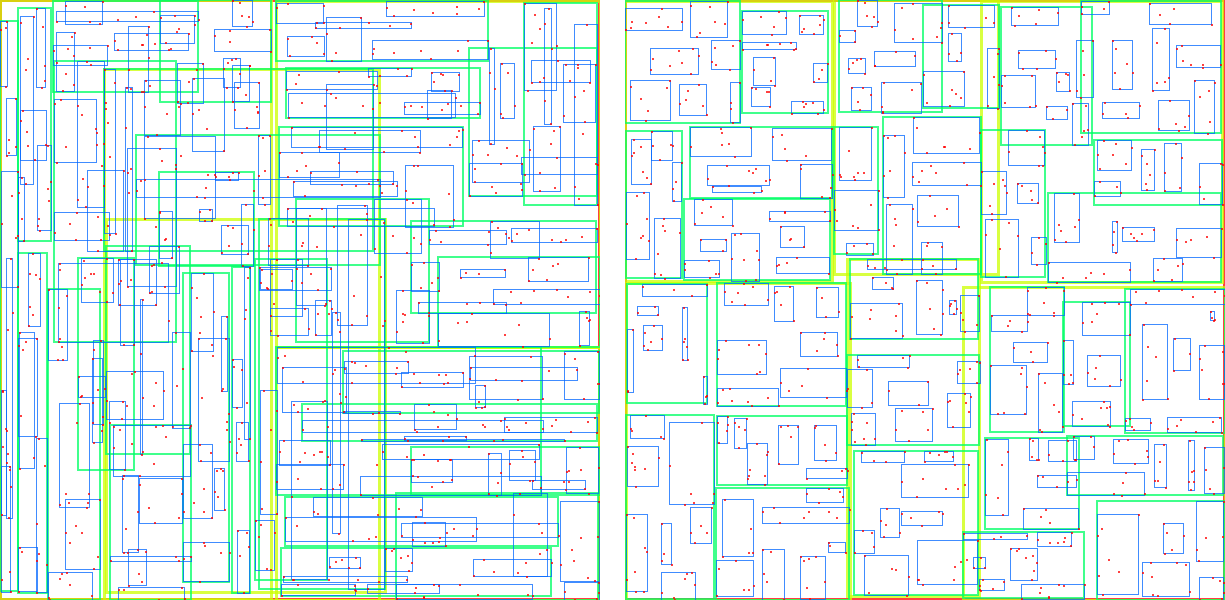
\includegraphics[width=1\textwidth]{vergleich-quad-star.png}
		\caption{Quadratischer- (links) und R*-Split (rechts) im Vergleich. (Bildquelle: \url{https://github.com/davidmoten/rtree})}
		\label{fig:vergleich-quad-star}
	\end{figure}

	Der R*-Baum betreibt sehr hohen Aufwand beim Hinzufügen und Löschen von Elementen, um eine gute Struktur zu bewahren. \Cref{fig:vergleich-quad-star} zeigt den gleichen Datensatz (mit gleicher Einfügereihenfolge), aber unterschiedlichen Split-Verfahren. Das Beispiel zeigt, wie positiv sich der Mehraufwand auswirkt. Mit R*-Split überschneiden sich die Verzeichnisrechtecke deutlich weniger, was schnellere Abfragen ermöglichen sollte und in den folgenden Benchmarks bestätigt wird.

	\subsubsection{Benchmarks} % (fold)
	\label{ssub:benchmarks}

	Die folgenden Benchmarks wurden von Beckmann, et.al. im Rahmen der ursprünglichen R*-Baum Veröffentlichung durchgeführt. Verglichen werden der originale R-Baum mit linearem, quadratischem und Greene-Split und der hier beschriebene R*-Baum. Die Parameter sind die für die jeweiligen Implementationen optimal gewählt \citep[vgl.][328]{Kriegel:2008}\footnote{$m=20\%$ (von $M$ maximalen Einträgen) für den linearen Split, quadratischer Split: $m=40\%$, Greene's-Split: $m=40\%$ und R*-Split: $m=40\%$}.

	Als Testdaten wurden fünf über verschiedene Verteilungen automatisch generierte Datensätze und ein realer Datensatz aus Höhenlinien gewählt (für eine genaue Beschreibung siehe \cite[328]{Kriegel:2008}). Die Daten wurden mit jeweils sieben verschiedenen Anfragen durchsucht und die Speicherzugriffe gemessen. Die Anfragen bestanden aus:
	\begin{description}
		\item[Point] Punkt-Anfrage ($1000\times$, gleich-verteilt im Raum)
		\item[Intersection] Suche nach allen Daten, welche die unterschiedlich großen Anfragerechtecke schneiden (je $100\times$, gleich-verteilt)
		\item[Contains] Suche nach allen Daten, die in den Anfragerechtecken komplett enthalten sind (ebenfalls je $100\times$, gleich-verteilt)
	\end{description}

	\begin{table}
	\caption{Alle Angaben sind relativ zu den Speicherzugriffen des R*-Baums.}
	\begin{tabularx}{\textwidth}{X|X|X|X|X|X|X|X}
		Point & \multicolumn{4}{c|}{Intersection} & \multicolumn{2}{c}{Contains \& Insert} \\
		 & $0.001\%$ & $0.01\%$ & $0.1\%$ & $1\%$ & $0.001\%$ & $0.01\%$ & 
	\end{tabularx}
	\end{table}
	
	% subsubsection benchmarks (end)

	\subsubsection{Weiterentwicklungen} % (fold)
	\label{ssub:weiterentwicklungen}

	Die Effizienz des R*-Baums nimmt ab fünf Dimensionen rapide ab \citep[vgl.][29]{Kriegel:2008}. Um auch höher dimensionalen Daten gerecht zu werden, existieren daher zahlreiche Weiterentwicklungen. Dazu gehört, wie eingangs erwähnt, der X-Baum, welcher darauf ausgelegt ist auch in höheren Dimensionen Überlappungen zu vermeiden \citep[vgl.][]{Kriegel:1996}.
	Andere Indizes bilden Näherungen der tatsächlichen Daten und führen Anfragen zunächst auf diesen aus (\emph{\enquote{Vector Approximation}}, siehe \cite{Gibas:2008} oder \cite{Daoudi:2008}). So wird der Zugriff auf Daten mit über 100 Dimensionen vergleichsweise effizient ermöglicht \citep[vgl.][]{Daoudi:2008}.
	
	% subsubsection weiterentwicklungen (end)

% section fazit (end)



% Anhang
%%%%%%%%%%%%%%%%%%%%%%%%%%%%%%%%%%%%%%%%%%%%%%%%%%%%%%%%%%%%%%%%%%%%
\newpage
\begin{appendix}

	\section*{Anhang}
	\addcontentsline{toc}{section}{Anhang}

	\section*{Abkürzungsverzeichnis} % (fold)
	\label{sub:abbreviations}

		\begin{acronym}[length]
			\acro{MBR}{Minimum bounding Rectangle}
	    \acro{SAM}{Spatial access methods}
	    \acro{PAM}{Point access methods}
	  \end{acronym}

	% section abbreviations (end)

	% Abbildungsverzeichnis
	% \listoffigures

	% Literaturverzeichnis
	%%%%%%%%%%%%%%%%%%%%%%%%%%%%%%%%%%%%%%%%%%%%%%%%%%%%%%%%%%%%%%%%%%%%b
	\nocite{*}							% include all bibtex entries from bibliography, even if they are not citied in the document

	\printbibliography

\end{appendix}

\end{document}
